\documentclass[
11pt, % The default document font size, options: 10pt, 11pt, 12pt
%codirector, % Uncomment to add a codirector to the title page
]{charter} 


% El títulos de la memoria, se usa en la carátula y se puede usar el cualquier lugar del documento con el comando \ttitle
\titulo{Interfaces Cerebro-Cloud para la predicción de actividades de imaginación motriz}

% Nombre del posgrado, se usa en la carátula y se puede usar el cualquier lugar del documento con el comando \degreename
%\posgrado{Carrera de Especialización en Sistemas Embebidos} 
%\posgrado{Carrera de Especialización en Internet de las Cosas} 
\posgrado{Carrera de Especialización en Inteligencia Artificial}
%\posgrado{Maestría en Sistemas Embebidos} 
%\posgrado{Maestría en Internet de las cosas}

% Tu nombre, se puede usar el cualquier lugar del documento con el comando \authorname
% IMPORTANTE: no omitir titulaciones ni tildación en los nombres, también se recomienda escribir los nombres completos (tal cual los tienen en su documento)
\autor{Ing. Freddy Julian Riascos Salas}

% El nombre del director y co-director, se puede usar el cualquier lugar del documento con el comando \supname y \cosupname y \pertesupname y \pertecosupname
\director{Mg. Ing. Jaime Andrés Riascos Salas}
\pertenenciaDirector{Potsdam Embodied Cognition Group PECoG} 
\codirector{} % para que aparezca en la portada se debe descomentar la opción codirector en los parámetros de documentclass
\pertenenciaCoDirector{FIUBA}

% Nombre del cliente, quien va a aprobar los resultados del proyecto, se puede usar con el comando \clientename y \empclientename
\cliente{Xprende}
\empresaCliente{Xprendetech S.A}
 
\fechaINICIO{4 de marzo de 2025}		%Fecha de inicio de la cursada de GdP \fechaInicioName
\fechaFINALPlan{22 de abril de 2025} 	%Fecha de final de cursada de GdP
\fechaFINALTrabajo{octubre de 2025}	%Fecha de defensa pública del trabajo final


\begin{document}

\maketitle
\thispagestyle{empty}
\pagebreak


\thispagestyle{empty}
{\setlength{\parskip}{0pt}
\tableofcontents{}
}
\pagebreak


\section*{Registros de cambios}
\label{sec:registro}


\begin{table}[ht]
\label{tab:registro}
\centering
\begin{tabularx}{\linewidth}{@{}|c|X|c|@{}}
\hline
\rowcolor[HTML]{C0C0C0} 
Revisión & \multicolumn{1}{c|}{\cellcolor[HTML]{C0C0C0}Detalles de los cambios realizados} & Fecha      \\ \hline
0      & Creación del documento                                 &\fechaInicioName \\ \hline
1      & Se completa hasta el 5 punto inclulsive                & 20 de marzo de 2025 \\ \hline
2      & Se completa hasta el 8 punto inclulsive               & 28 de marzo de 2025 \\ \hline
%1      & Se completa hasta el punto 5 inclusive                & {día} de {mes} de 202X \\ \hline
%2      & Se completa hasta el punto 9 inclusive
%		  Se puede agregar algo más \newline
%		  En distintas líneas \newline
%		  Así                                                    & {día} de {mes} de 202X \\ \hline
%3      & Se completa hasta el punto 12 inclusive                & {día} de {mes} de 202X \\ \hline
%4      & Se completa el plan	                                 & {día} de {mes} de 202X \\ \hline

% Si hay más correcciones pasada la versión 4 también se deben especificar acá

\end{tabularx}
\end{table}

\pagebreak



\section*{Acta de constitución del proyecto}
\label{sec:acta}

\begin{flushright}
Buenos Aires, \fechaInicioName
\end{flushright}

\vspace{2cm}

Por medio de la presente se acuerda con el \authorname\hspace{1px} que su Trabajo Final de la \degreename\hspace{1px} se titulará ``\ttitle'' y consistirá en \textit{evaluar una interfaz cerebro-computadora (Brain-Computer Interface}, BCI) \textit{con soporte en la nube para la detección de patrones de imaginación motriz}. El trabajo tendrá un presupuesto preliminar estimado de 600 horas y un costo estimado de \$25000, con fecha de inicio el \fechaInicioName\hspace{1px} y fecha de presentación pública el \fechaFinalName.

Se adjunta a esta acta la planificación inicial.

\vfill

% Esta parte se construye sola con la información que hayan cargado en el preámbulo del documento y no debe modificarla
\begin{table}[ht]
\centering
\begin{tabular}{ccc}
\begin{tabular}[c]{@{}c@{}}Dr. Ing. Ariel Lutenberg \\ Director posgrado FIUBA\end{tabular} & \hspace{2cm} & \begin{tabular}[c]{@{}c@{}}\clientename \\ \empclientename \end{tabular} \vspace{2.5cm} \\ 
\multicolumn{3}{c}{\begin{tabular}[c]{@{}c@{}} \supname \\ Director del Trabajo Final\end{tabular}} \vspace{2.5cm} \\
\end{tabular}
\end{table}




\section{1. Descripción técnica-conceptual del proyecto a realizar}
\label{sec:descripcion}

% ELIMINAR \begin{consigna}{red} y \end{consigna}{red} en las secciones que vayan completando para cada entrega parcial.
Las interfaces cerebro-computadora (\textit{Brain-Computer Interfaces}, BCI) han emergido como una tecnología innovadora que permite la comunicación directa entre el cerebro humano y dispositivos externos.
En particular, la predicción de actividades de imaginación motriz a través de BCI han cobrado relevancia en campos que varían desde la rehabilitación, robótica, control de protésis hasta sistemas domóticos, videojuegos y realidad virtual.

La integración de las BCI con tecnologías en la nube permite el almacenamiento, procesamiento y análisis eficiente de grandes volúmenes de datos cerebrales. Esto favorece la aplicación de algoritmos avanzados de aprendizaje automático y mejora la precisión de la interpretación de señales cerebrales.

\textbf{1.1 Conceptos fundamentales}

Interfaces cerebro-computadora

Los BCI son sistemas que registran la actividad cerebral mediante técnicas como la electroencefalografía (EEG) y traducen estas señales en comandos computacionales. Existen distintos tipos de BCI:
\begin{itemize}
	\item Invasivas: electrodos implantados directamente en el cerebro.
	\item No invasivas: uso de sensores externos como EEG, MEG o fNIRS.
\end{itemize}

Imaginación motriz

La imaginación motriz se refiere a la capacidad de representar mentalmente movimientos sin ejecutarlos físicamente. Durante este proceso, se activan patrones específicos en la corteza motora, los cuales pueden ser detectados mediante EEG y utilizados para el control de dispositivos externos.

Computación en la nube y BCI

El uso de servicios en la nube permite procesar grandes volúmenes de datos EEG en tiempo real obteniendo beneficios como:
\begin{itemize}
	\item Almacenamiento y procesamiento escalable de datos cerebrales.
	\item Acceso remoto para análisis colaborativo.
	\item Implementación de modelos de aprendizaje automático en infraestructura distribuida.
\end{itemize}

\textbf{1.2 Problema actual}

Al presente, las personas con discapacidades motoras severas enfrentan grandes dificultades en la interacción con su entorno. Los sistemas actuales de BCI presentan limitaciones en términos de precisión, latencia, accesibilidad, recopilación,
análisis y clasificación de las señales EEG. Normalmente, estos datos se encuentran contaminados por distintos artefactos biológicos, tales como señales cardíacas, respiratorias o músculos, como también por ruidos externos.

Así mismo, la dimensión de estos datos, dada por la cantidad de canales y señal de tiempo, crea una problema de procesamiento y dimensionalidad. Todas estas dificultades evitan que el clasificador reciba características latentes de la señal y así realizar la predicción de forma adecuada y rápida.

\textbf{1.3 Solución propuesta}

La interfaz Cerebro-Cloud sugerida integra un modelo de predicción basado en aprendizaje automático con una arquitectura en la nube que permita la adquisición, procesamiento y transmisión de señales cerebrales en tiempo real. Esto proporcionará una solución más precisa, escalable y accesible para el control
de dispositivos mediante imaginación motriz.



En comparación con el estado del arte actual, la solución se destaca en:

\begin{itemize}
	\item Precisión mejorada: uso de modelos de inteligencia artificial optimizados para la interpretación de señales eléctricas (electroencefalografía, EEG).
	\item Reducción de latencia: procesamiento distribuido en la nube.
	\item Accesibilidad: plataforma escalable con acceso a la información para usuarios y especialistas.
\end{itemize}

Este interfaz BCI-Cloud tiene como objetivo mejorar la calidad de vida de personas con discapacidades motoras
al proporcionar una herramienta en la nube para la comunicación y control de dispositivos protésicos.

El proyecto se enmarca dentro de un programa de innovación tecnológica de la empresa \clientename, que cuenta con financiamiento para su ejecución.

\textbf{1.4 Descripción funcional y diagrama en bloques}

La solución propuesta consta de los siguientes módulos principales:
\begin{itemize}
	\item Adquisición de señales EEG: sensores no invasivos capturan la actividad cerebral del usuario.
	\item Preprocesamiento de datos: filtrado y eliminación de ruido en las señales EEG.
	\item Modelo de predicción: algoritmos de aprendizaje automático analizan los datos y determinan la intención motriz.
	\item Transmisión en la nube: los datos procesados se envían a servidores remotos para análisis y almacenamiento.
	\item Interfaz usuario-dispositivo: una interfaz que traduce la predicción en comandos para dispositivos externos, como prótesis o interfaces de control.
\end{itemize}

En la figura 1 se presenta el diagrama de bloques del sistema BCI-Cloud. Se observa que el usuario inicial genera datos con el sensor EEG. Luego envía los datos a un sistema de preprocesamiento. 
Una vez que los datos se encuentran óptimos se envian a la nube. Seguidamente el modelo seleccionado se entrena. Finalmente el modelo predice el movimiento imaginado en la interfaz de usaurio.

\begin{figure}[htpb]
\centering 
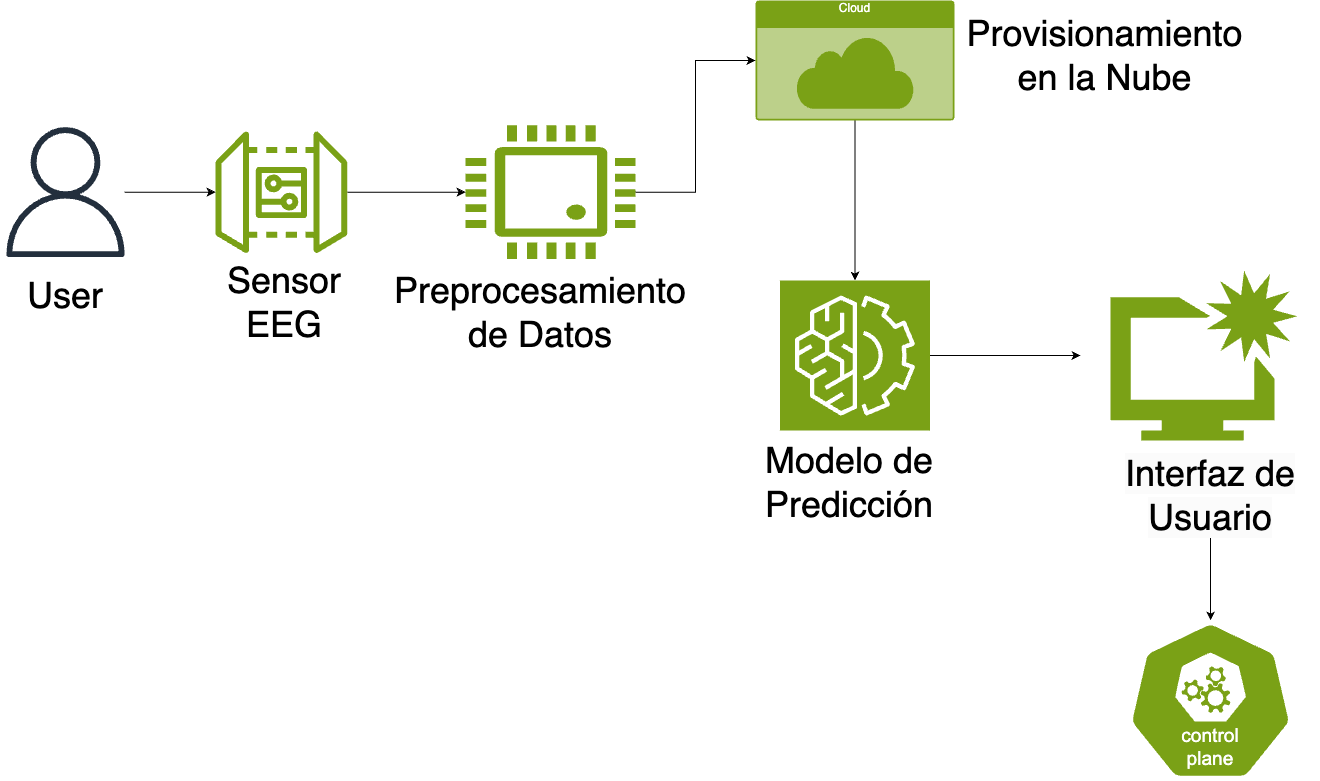
\includegraphics[width=.65\textwidth]{./Figuras/block_diagram.png}
\caption{Diagrama del sistema BCI-Cloud.}
\label{fig:diagBloques}
\end{figure}

\vspace{25px}

% ELIMINAR \begin{consigna}{red} y \end{consigna}{red} en las secciones que vayan completando para cada entrega parcial.

\section{2. Identificación y análisis de los interesados}
\label{sec:interesados}

A continuación, se presentan los principales actores involucrados en el desarollo del proyecto y su respectiva función:
 
\begin{table}[ht]
%\caption{Identificación de los interesados}
%\label{tab:interesados}
\begin{tabularx}{\linewidth}{@{}|l|X|X|l|@{}}
\hline
\rowcolor[HTML]{C0C0C0} 
Rol           & Nombre y Apellido & Organización 	& Puesto 	\\ \hline
Cliente       & Ing. Miguel Amaya       &\empclientename	& -       	\\ \hline
Responsable   & \authorname       & FIUBA        	& Alumno 	\\ \hline
Orientador    & \supname	      & \pertesupname 	& Director del Trabajo Final \\ \hline
Usuario final & Paciente          & -             	& -        	\\ \hline
\end{tabularx}
\end{table}

A continuación las principales características de cada interesado.
 
\begin{itemize}
	\item Orientador: el Mg. Ing. Andrés Salas es experto en desarrollar interfaces cerebro-maquina y dará orientación con la definición de los requerimientos y el desarrollo del sistema BCI-Cloud.
	\item Usuario final: usuario con discapacidad motora severa, quien se beneficiaría directamente del control del dispositivo y la interfaz.
\end{itemize}

% ELIMINAR \begin{consigna}{red} y \end{consigna}{red} en las secciones que vayan completando para cada entrega parcial.
\section{3. Propósito del proyecto}
\label{sec:proposito}
La intención del proyecto es diseñar y desarrollar una plataforma basada en BCI-Cloud que facilite la predicción de actividades de imaginación motriz en personas con discapacidades motoras severas. A través de la integración de inteligencia artificial y computación en la nube, se busca ofrecer una solución innovadora que permita mejorar la interacción con el entorno mediante el control preciso de dispositivos electrónicos y protésicos.

\section{4. Alcance del proyecto}
\label{sec:alcance}

El proyecto comprenderá los siguientes componentes:
\begin{itemize}
	\item Modelo de predicción basado en algoritmos de aprendizaje automático para la interpretación de señales EEG. Se evaluarán distintos modelos como CNNs, RNNs y \textit{Transformers} para determinar el que mejor performe en términos de precisión y latencia.
	\item Datos adquiridos de sensores EEG, que se utilizarán para entrenar y validar el modelo. Se garantizará que la adquisición de datos cumpla con estándares de calidad y se preprocesen para eliminar ruido.
	\item Código de la infraestructura en la nube.
	\item Documentación técnica y científica, que detalla el diseño, implementación y validación del sistema.
	\item Pruebas y validaciones realizadas con usuarios objetivo para evaluar el desempeño y precisión del modelo. Se incluirán métricas clave que garanticen el óptimo desempeño del sistema.
	\item Desarrollo y entrenamiento del modelo de predicción de actividades de imaginación motriz, con comparaciones entre distintos enfoques de inteligencia artificial.
	\item Integración con una infraestructura en la nube escalable y segura en \textit{Amazon Web Services}.
	\item Adquisición y procesamiento de señales cerebrales mediante sensores EEG.
	\item Evaluación del sistema con usuarios finales para validar su precisión y usabilidad.
	\item Generación de documentación técnica para futuras mejoras e implementación.
	\item Optimización del procesamiento en la nube para reducir latencia y mejorar la eficiencia del sistema.
\end{itemize}
El presente proyecto no incluye:
\begin{itemize}
	\item Desarrollo de hardware EEG propio. Para ello se utilizarán dispositivos comerciales disponibles en el mercado.
	\item Implementación de interfaces cerebro-máquina más allá de la imaginación motriz.
	\item Integración con sistemas de salud o bases de datos clínicas.
\end{itemize}

% ELIMINAR \begin{consigna}{red} y \end{consigna}{red} en las secciones que vayan completando para cada entrega parcial.


\section{5. Supuestos del proyecto}
\label{sec:supuestos}
\begin{itemize}
	\item Disponibilidad de datos EEG de calidad: se asume que los datos recopilados mediante sensores EEG serán suficientes y de calidad adecuada para el entrenamiento del modelo sin necesidad de un preprocesamiento excesivo.
	\item Recursos computacionales: se cuenta con acceso a instancias de cómputo en la nube, tales como las brindadas por \textit{Amazon Web Services}, que permitan el entrenamiento y despliegue del modelo de inteligencia artificial sin limitaciones de procesamiento o almacenamiento.
	\item Factibilidad técnica de integración: se considera viable la integración entre los sensores EEG, la infraestructura en la nube y la interfaz de usuario.
	\item Condiciones regulatorias favorables: no existen restricciones legales o normativas que impidan la recopilación y procesamiento de datos EEG.
\end{itemize}

% ELIMINAR \begin{consigna}{red} y \end{consigna}{red} en las secciones que vayan completando para cada entrega parcial.

\section{6. Product backlog}
\label{sec:backlog}
\begin{enumerate}
	\item Épica 1 - Adquisición y procesamiento de datasets EEG
	\begin{enumerate}
		\item HU1 
		
		Como ingeniero, quiero obtener señales EEG desde datasets públicos para alimentar el modelo de predicción.\newline
		
		
		Dificultad: 5
		
		Complejidad: 4 
		
		Incertidumbre: 3
		
		Suma: 12 → \textit{Story Points}: 13
		
		Prioridad: 1\newline
		
		
		\item HU2
		
		Como ingeniero, quiero que las señales EEG sean filtradas y normalizadas automáticamente para mejorar la calidad del entrenamiento del modelo.\newline

		Dificultad: 4 
		
		Complejidad: 2 
		
		Incertidumbre: 2 
		
		Suma: 8 → \textit{Story Points}: 8

		Prioridad: 2\newline

		
	\end{enumerate}
	\item Épica 2 - Inteligencia artificial y modelado
	\begin{enumerate}
		\item HU3
		
		Como ingeniero, quiero entrenar un modelo de inteligencia artificial con señales EEG preprocesadas para predecir actividades de imaginación motriz con alta precisión.\newline
		
		Dificultad: 5
		
		Complejidad: 5
		
		Incertidumbre: 4
		
		Suma: 14 → \textit{Story Points}: 21
		
		Prioridad: 3\newline
		
		\item HU4
		
		Como ingeniero, quiero optimizar el modelo de inteligencia artificial para que el tiempo de respuesta sea menor a 5000 ms, una precisión de 80\% y mejorar la experiencia del usuario.\newline
		
		Dificultad: 4
		
		Complejidad: 3
		
		Incertidumbre: 3
		
		Suma: 10 → \textit{Story Points}: 13

		Prioridad: 4\newline
	\end{enumerate}
	\item Épica 3 - Infraestructura en la nube
	\begin{enumerate}
		\item HU5
		
		Como ingeniero, quiero que el procesamiento de datos EEG ocurra en \textit{Amazon Web Services} AWS Lambda para mejorar la escalabilidad del sistema.\newline
		
		Dificultad: 5
		
		Complejidad: 4
		
		Incertidumbre: 3
		
		Suma: 12 → \textit{Story Points}: 13

		Prioridad: 5\newline
		
		\item HU6
		
		Como ingeniero, quiero una API REST para conectar los dispositivos EEG con la nube y enviar los datos en tiempo real.\newline
		
		Dificultad: 4
		
		Complejidad: 3
		
		Incertidumbre: 3
		
		Suma: 10 → \textit{Story Points}: 13

		Prioridad: 6\newline
	\end{enumerate}
	\item Épica 4 - Interfaz de usuario y seguridad
	\begin{enumerate}
		\item HU7
		
		Como usuario final, quiero visualizar mis señales EEG en una interfaz gráfica para entender cómo se interpretan mis actividades cerebrales.\newline
		
		Dificultad: 5
		
		Complejidad: 3
		
		Incertidumbre: 2
		
		Suma: 10 → \textit{Story Points}: 13
		
		Prioridad: 7\newline
		
		\item HU8
		
		Como ingeniero, quiero que los datos EEG sean almacenados y transmitidos de manera segura para cumplir con las normativas de privacidad.\newline
		
		Dificultad: 5
		
		Complejidad: 5
		
		Incertidumbre: 2
		
		Suma: 12 → \textit{Story Points}: 13

		Prioridad: 8\newline
	\end{enumerate}
\end{enumerate}

\section{7. Criterios de aceptación de historias de usuario}
\label{sec:criteriosAceptacion}
\begin{enumerate}
	\item Épica 1 - Adquisición y procesamiento de datasets EEG

	\begin{enumerate}
		\item Criterios de aceptación HU1
			\begin{itemize}
				\item Se deben verificar al menos 2 repositorios públicos de datasets que estén accesibles y disponibles para su descarga.
				\item Los datos deben almacenarse automáticamente en una ruta definida del proyecto, sin intervención manual.
				\item Se debe validar que el formato de los datos descargados sea compatible con la tubería de procesamiento.
				\item Los datos almacenados se deben organizar en una estructura jerárquica que difiera entre los repositorios consultados.
				\item Se debe crear un archivo de documentación que describa la información de los datos, tales como fuentes usadas, formatos y cantidad de muestras.
			\end{itemize}
			  
		\item Criterios de aceptación HU2
			\begin{itemize}
			\item Se debe aplicar al menos un filtro a las señales EEG para eliminar frecuencias no deseadas.
			\item Los datos deben estar escalados y asegurar que todos los canales estén en la misma escala.
			\item Se debe crear un archivo de documentación que describa los filtros aplicados, método de normalización y duración del proces.
			\item Se debe crear un archivo de documentación que describa los filtros aplicados, método de normalización y duración del proces.
			\item Se debe generarse un gráfico comparando la señal original y la procesada conocer la efectividad del filtrado y normalización.
			\end{itemize}
	\end{enumerate}
	\item Épica 2 - Inteligencia artificial y modelado
	\begin{enumerate}
		\item Criterios de aceptación HU3
			\begin{itemize}
			\item  El modelo de predicción debe alcanzar una precisión mínima del 85\% en validación cruzada.
			\item  Se deben entrenar al menos tres arquitecturas y seleccionar la mejor.
			\item  Se deben generar logs detallados del proceso de entrenamiento con métricas de desempeño.
			\end{itemize}
		\item Criterios de aceptación HU4
			\begin{itemize}
			\item  El modelo optimizado debe tener un tiempo de inferencia menor a 5000 ms.
			\item  La implementación debe utilizar hardware optimizado en la nube.
			\item  Se debe medir la latencia en diferentes condiciones de carga y garantizar estabilidad.
			\item Los resultados de predicción deben ser accesibles en tiempo real a través de una API REST.
			\end{itemize}
	\end{enumerate}
	\item Épica 3 - Infraestructura en la nube
	\begin{enumerate}
		\item Criterios de aceptación HU5
			\begin{itemize}
			\item  La infraestructura debe ser escalable, permitiendo hasta 1000 eventos concurrentes.
			\item  Se debe garantizar un 85.9\% de disponibilidad del servicio en producción.
			\item  \textit{Amazon Web Services} Lambda debe procesar eventos EEG en tiempo real con ejecución máxima de 15 segundos.
			\end{itemize}
		\item Criterios de aceptación HU6
			\begin{itemize}
			\item  La API REST debe permitir la recepción de datos EEG con un \textit{endpoint} dedicado.
			\item  Debe incluir autenticación y autorización mediante \textit{tokens} \textit{Json Web Tokens}.
			\item  La API REST debe responder con código 200 OK en menos de 300 ms en condiciones normales.
			\item La documentación de la API REST debe estar disponible con ejemplos de uso.
			\end{itemize}
	\end{enumerate}
	\item Épica 4 - Interfaz de usuario y seguridad
	\begin{enumerate}
		\item Criterios de aceptación HU7
			\begin{itemize}
			\item La interfaz debe permitir visualizar las señales EEG en gráficos.
			\item Se debe permitir la exportación de datos en formatos CSV y JSON.
			\end{itemize}
		\item Criterios de aceptación HU8
			\begin{itemize}
			\item Los datos EEG deben ser cifrados en tránsito y en reposo.
			\item El sistema debe incluir una política de retención y eliminación de datos.
			\end{itemize}
	\end{enumerate}
\end{enumerate}

\section{8. Fases de CRISP-DM}
\label{sec:entregables}

Comprensión del negocio

Objetivo: desarrollar un modelo de inteligencia artificial que analice señales EEG para predecir la intención de movimiento en usuarios, lo que facilitarían aplicaciones en neurorehabilitación y control de dispositivos.

Valor agregado: automatización del análisis de señales cerebrales para mejorar la accesibilidad a tecnologías BCI.

Métricas de éxito: 
\begin{itemize}
	\item Precisión mínima del modelo: 85\%.
	\item Latencia de predicción menor a 5000 ms.
	\item Disponibilidad del sistema: 85\% en producción.
	\item Cumplimiento de normativas de seguridad.
\end{itemize}

Comprensión de los datos

\begin{itemize}
	\item Tipo de datos: señales de series temporales EEG obtenidas de dispositivos de adquisición neurofisiológica.
	\item Fuentes: sensores EEG comerciales como \textit{OpenBCI}, \textit{Emotiv} o bases de datos públicas.
	\item Cantidad: al menos 100,000 registros diarios procesados en \textit{Amazon Web Services}.
	\item Calidad: se esperan encontrar ruidos, artefactos musculares y variabilidad intersujeto.
\end{itemize}

Preparación de los datos

Las características claves a tener en cuenta para las señales EEG son:

\begin{itemize}
	\item Bandas de frecuencia.
	\item Espectrogramas de señales EEG.
	\item Características temporales obtenidas con algoritmos de \textit{STFT} y \textit{Wavelet}.
\end{itemize}

Las transformaciones que podrían ser requeridas para las señales EEG son:
\begin{itemize}
	\item Filtrado pasa bandas.
	\item Normalización de señales.
	\item Eliminación de artefactos usando algoritmos de análisis de componentes principales.
\end{itemize}

Modelado

El problema se define como una clasificación de señales EEG para la predicción de imaginación motriz.
Mientras las arquitecturas candidatas para este problema son redes neuronales como CNNs, RNNs y \textit{Transformers}.

Evaluación del modelo

Se podría utilizar el \textit{acurracy} para conocer la precisión de aciertos en la predicción de clases de imaginación motriz. Además el \textit{F1-score} y la matriz de confusión para obtener
el balance entre precisión y exhaustividad y los falsos positivos y falsos negativos. 

Despliegue del modelo

El modelo se implementará con un sistema basado en la nube con \textit{Amazon Web Services} Lambda para procesamiento, una API REST para enviar los datos a la nube y una fuente
de almacenamiento que proporcione un costo beneficio en los datos durante el tiempo.

\section{9. Desglose del trabajo en tareas}
\label{sec:wbs}

\begin{table}[htpb]
\centering
\begin{tabularx}{\linewidth}{@{}|X|X|c|c|@{}}
\hline
\rowcolor[HTML]{C0C0C0}
Historia de usuario & Tarea técnica & Estimación & Prioridad \\ \hline
HU1 & Investigación y selección de datasets públicos relevantes & 6 h & Alta \\ \hline
HU1 & Descarga manual y validación de estructura de archivos EEG del primer dataset & 6 h & Alta \\ \hline
HU1 & Implementación de script de descarga automática para datasets seleccionados	 & 8 h & Alta \\ \hline
HU1 & Estudio y análisis de metadatos disponibles en los datasets	 & 6 h & Media \\ \hline
HU1 & Conversión y unificación de formatos		 & 8 h & Media \\ \hline
HU1 & Verificación de integridad de los archivos descargados			 & 4 h & Alta \\ \hline
HU1 & Almacenamiento y organización de señales EEG				 & 6 h & Alta \\ \hline
HU1 & Documentación del proceso de adquisición				 & 6 h & Baja \\ \hline
HU1 & Evaluación legal/licencia de uso de los datasets				 & 4 h & Media \\ \hline
HU1 & Generación de logs y reportes de adquisición				 & 4 h & Baja \\ \hline
HU2 & Implementación de función de filtrado por banda					 & 8 h & Alta \\ \hline
HU2 & Implementación de detección y corrección de artefactos simples					 & 6 h & Alta \\ \hline
HU2 & Implementación de métodos de normalización 					 & 6 h & Alta \\ \hline
HU2 & Diseño de pipeline automático de procesamiento por lote					 & 8 h & Alta \\ \hline
HU2 & Pruebas con señales reales y comparación visual					 & 6 h & Media \\ \hline
HU2 & Generación de logs por archivo procesado				 & 4 h & Baja \\ \hline
HU2 & Creación de gráficas de validación por dataset					 & 6 h & Media \\ \hline
HU2 & Evaluación de calidad de la señal post-procesamiento					 & 6 h & Media \\ \hline
HU2 & Desarrollo de manejo de errores en procesamiento					 & 8 h & Media \\ \hline
HU2 & Documentación del pipeline de procesamiento					 & 8 h & Baja \\ \hline
HU2 & Generación de logs y reportes de adquisición				 & 4 h & Baja \\ \hline
HU3 & Selección de señales EEG preprocesadas para el entrenamiento						 & 6 h & Alta \\ \hline
HU3 & Estudio de modelos de clasificación adecuados para señales EEG					 & 8 h & Alta \\ \hline
HU3 & Implementación del primer modelo base (baseline)					 & 8 h & Alta \\ \hline
HU3 & Implementación del segundo modelo 	(alternativo)			 & 8 h & Alta \\ \hline
... & ... & ... & ... \\ \hline
\end{tabularx}
\end{table}



\section{10. Diagrama de Gantt}
\label{sec:wbs}
\begin{enumerate}
\item Formación técnica (140h)
	\begin{enumerate}
	\item Estudio del estado del arte. (40h)
	\item Capacitación en señales de series de tiempo EGG. (40h)
	\item Capacitación en el uso de BCI basada en imaginación motora. (40h)
	\item Capacitación en el uso de AWS para el procesamiento y despleigue de los modelos. (20h)
	\end{enumerate}
\item Preparación de los datos para desarrollar el modelo (20h)
	\begin{enumerate}
	\item Busqueda de fuentes. (4h)
	\item Implementación de descarga de datos (4h)
	\item Preparación de los datos. (12h)
	\end{enumerate}
\item Busqueda e implementación de 3 modelos de aprendizaje(124h)
	\begin{enumerate}
	\item Estudio de bibliografía del primero modelo. (10h)
	\item Implementación del primero modelo. (40h)
	\item Estudio de bibliografía del segundo modelo. (10h)
	\item Implementación del segundo modelo. (20h)
	\item Estudio de bibliografía del tercer modelo. (10h)
	\item Implementación del tercer modelo. (20h)
	\item Análisis de ventajas y desventajas de cada implementación. (10h)
	\item Selección del mejor modelo basado en el análisis de cada implementación. (4h)
	\end{enumerate}
\item Implementación de la infraestructura en AWS(120h)
	\begin{enumerate}
	\item Configuración del almacenamiento de datos. (20h)
	\item Configuración de la arquitectura escalable. (20h)
	\item Configuración del procesamiento de datos. (20h)
	\item Configuración de la seguridad en los datos. (20h)
	\item Configuración de la politica de retención y eliminación de datos. (20h)
	\item Añadir los \textit{endpoints} para comunicación de los datos. (10h)
	\item Elaboración de la documentación del código de infraestructura (10h)
	\end{enumerate}
\item Implementación de la interfaz de usuario (100h)
	\begin{enumerate}
	\item Desarrollo de código para exportar datos. (40h)
	\item Desarrollo de código para visualizar las señales EEG. (40h) 
	\item Desarrollo de código para visualizar la predicción de imaginación motora. (10h)
	\item Elaboración de la documentación del código de interfaz de usuario. (10h)
	\end{enumerate}
\item Elaboración de la documentación y presentación (56h)
	\begin{enumerate}
	\item Escritura de las memorias del proyecto. (40h)
	\item Elaboración de la presentación final. (20)
	\item Ensayo de la presentación final. (16h)
	\end{enumerate}

\end{enumerate}
Cantidad total de horas: 600.
\section{10. Diagrama de Activity On Node}
\label{sec:AoN}
\begin{figure}[htpb]
\centering 
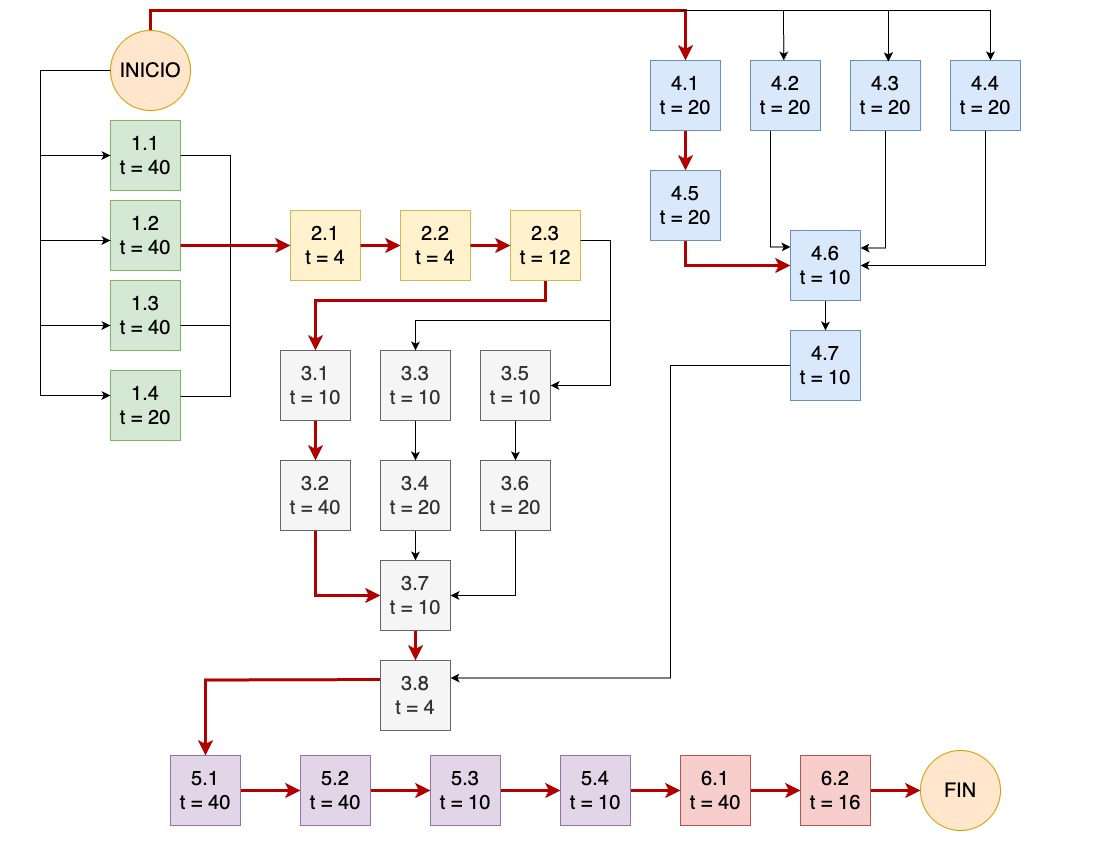
\includegraphics[width=.8\textwidth]{./Figuras/AoN-project.jpg}
\caption{Diagrama de \textit{Activity on Node}.}
\label{fig:AoN}
\end{figure}

En la figura 2 se visualiza el diagrama de \textit{Activity on Node} del proyecto. Se indica en color rojo el camino crítico y el tiempo de cada tarea esta en horas.

\section{11. Diagrama de Gantt}
\label{sec:gantt}

\begin{consigna}{red}
\begin{landscape}
\begin{figure}[htpb]
\centering 
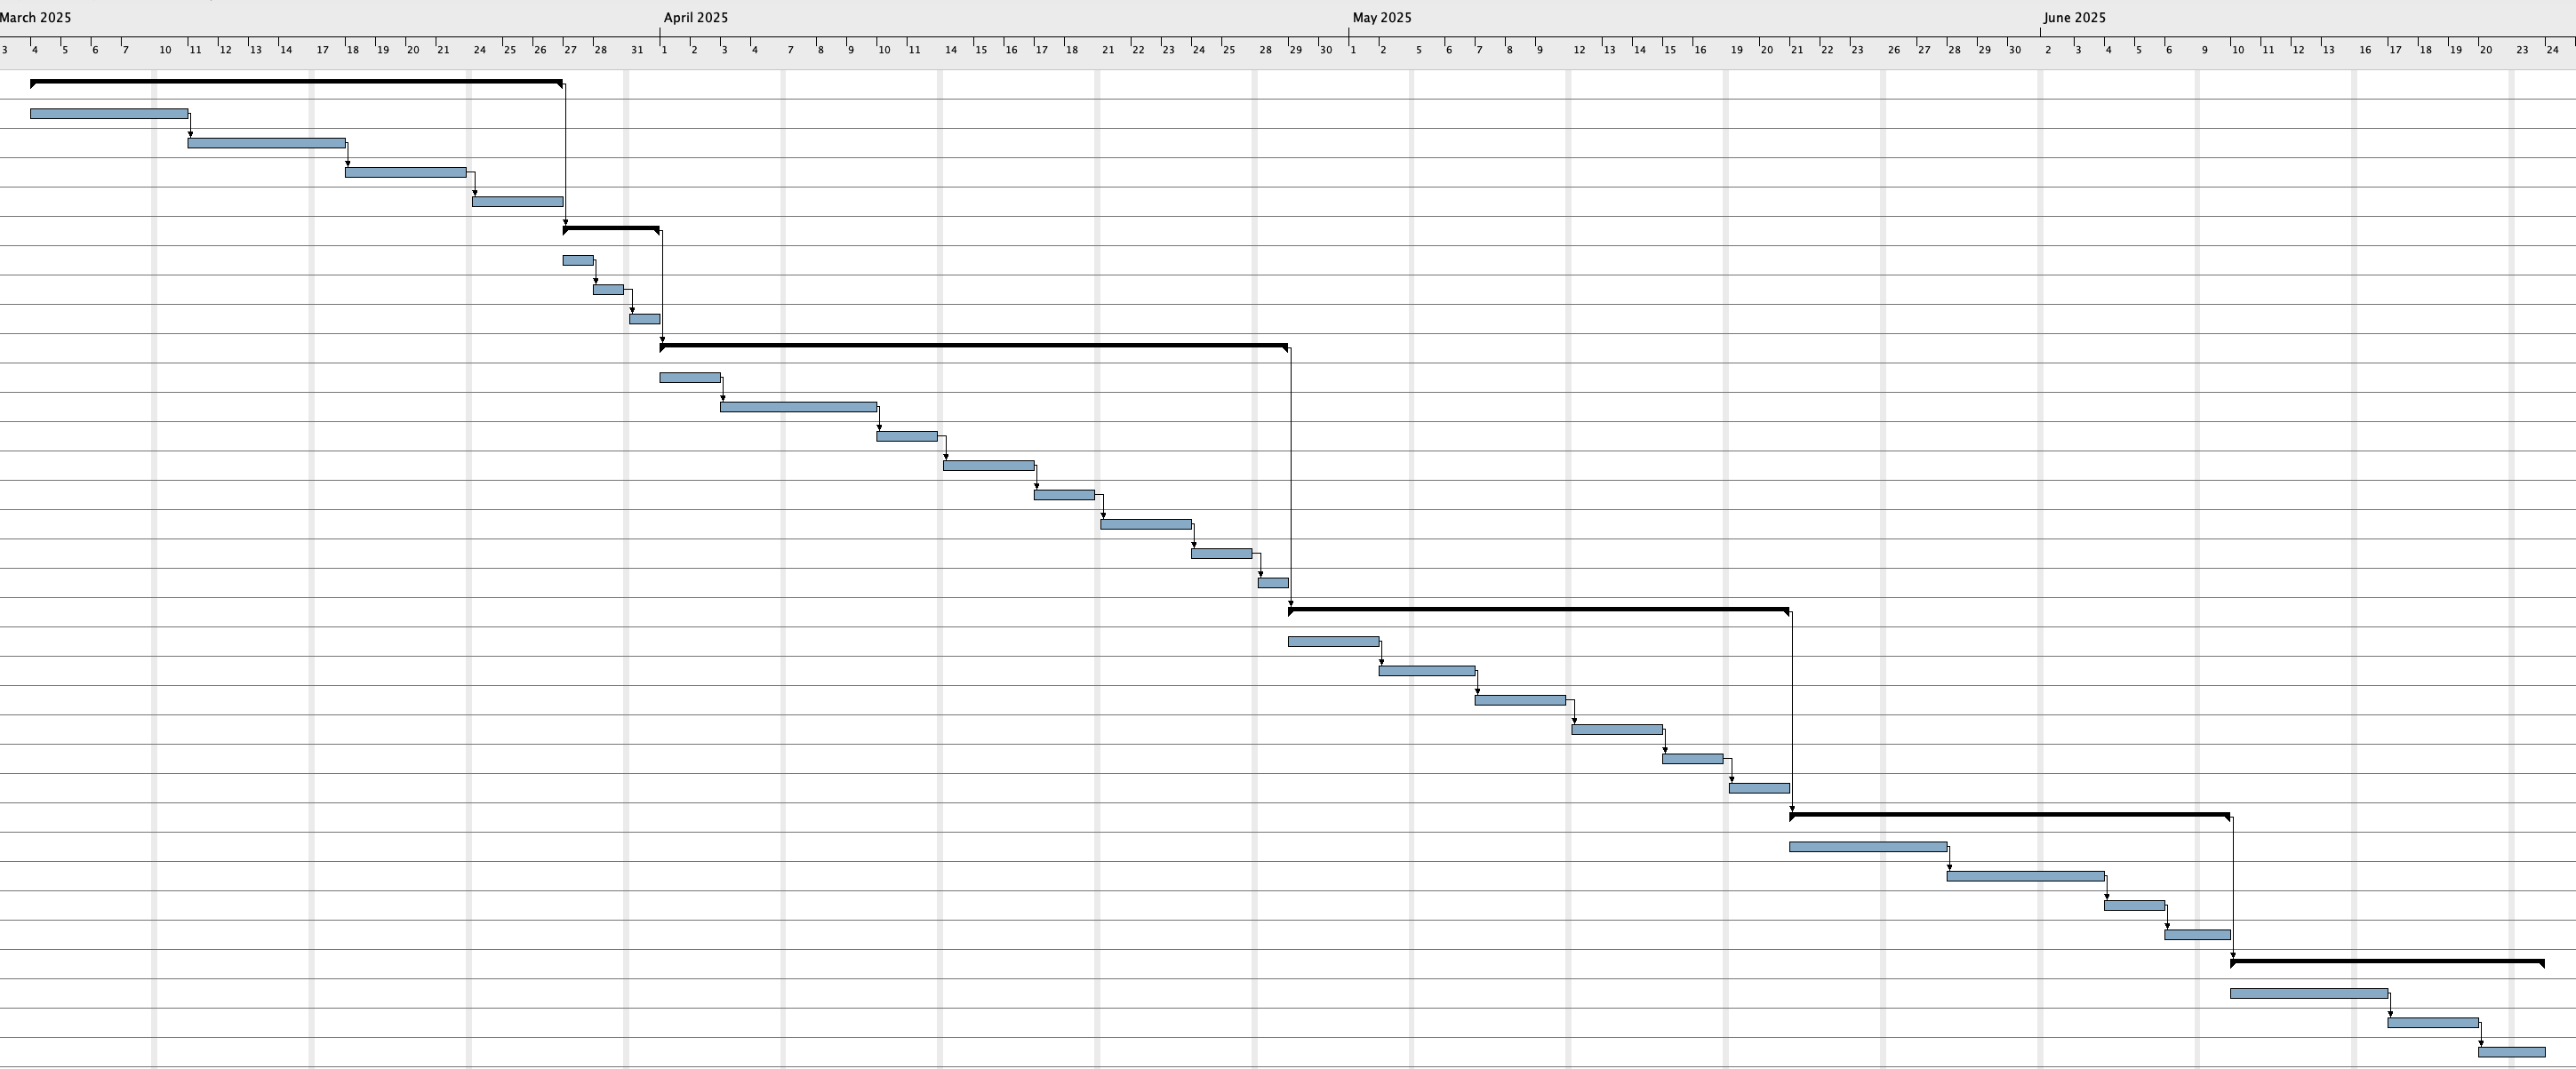
\includegraphics[height=.85\textheight]{./Figuras/bad-format-grant.png}
\caption{Diagrama de Gantt (apaisado).} %Modificar este título acorde.
\label{fig:diagGantt}
\end{figure}

\end{landscape}

\end{consigna}


\section{12. Presupuesto detallado del proyecto}
\label{sec:presupuesto}

\begin{consigna}{red}

\end{consigna}

\begin{table}[htpb]
\centering
\begin{tabularx}{\linewidth}{@{}|X|c|r|r|@{}}
\hline
\rowcolor[HTML]{C0C0C0} 
\multicolumn{4}{|c|}{\cellcolor[HTML]{C0C0C0}COSTOS DIRECTOS} \\ \hline
\rowcolor[HTML]{C0C0C0} 
Descripción & 
  \multicolumn{1}{c|}{\cellcolor[HTML]{C0C0C0}Cantidad} &
  \multicolumn{1}{c|}{\cellcolor[HTML]{C0C0C0}Valor unitario} &
  \multicolumn{1}{c|}{\cellcolor[HTML]{C0C0C0}Valor total} \\ \hline
 Honoracios del ingeniero&
  \multicolumn{1}{c|}{600} &
  \multicolumn{1}{c|}{\$40} &
  \multicolumn{1}{c|}{\$24000} \\ \hline
 Computación en la nube&
  \multicolumn{1}{c|}{} &
  \multicolumn{1}{c|}{} &
  \multicolumn{1}{c|}{\$200} \\ \hline
  Almacenamiento en la nube AWS&
  \multicolumn{1}{c|}{}&
  \multicolumn{1}{c|}{}&
  \multicolumn{1}{c|}{\$50}\\ \hline
\multicolumn{1}{|l|}{} &
   &
   &
   \\ \hline
\multicolumn{3}{|c|}{SUBTOTAL} &
  \multicolumn{1}{c|}{\$24250} \\ \hline
\rowcolor[HTML]{C0C0C0} 
\multicolumn{4}{|c|}{\cellcolor[HTML]{C0C0C0}COSTOS INDIRECTOS} \\ \hline
\rowcolor[HTML]{C0C0C0} 
Descripción &
  \multicolumn{1}{c|}{\cellcolor[HTML]{C0C0C0}Cantidad} &
  \multicolumn{1}{c|}{\cellcolor[HTML]{C0C0C0}Valor unitario} &
  \multicolumn{1}{c|}{\cellcolor[HTML]{C0C0C0}Valor total} \\ \hline
\multicolumn{1}{|l|}{15\% de costos directos} &
   &
   &
   \multicolumn{1}{c|}{\$3638} \\ \hline
   
\multicolumn{1}{|l|}{} &
   &
   &
   \\ \hline
\multicolumn{1}{|l|}{} &
   &
   &
   \\ \hline
\multicolumn{3}{|c|}{SUBTOTAL} &
\multicolumn{1}{c|}{\$3638} \\ \hline
\rowcolor[HTML]{C0C0C0}
\multicolumn{3}{|c|}{TOTAL} &
\multicolumn{1}{c|}{\$27888} \\ \hline
\end{tabularx}%
\end{table}


\section{13. Gestión de riesgos}
\label{sec:riesgos}

\begin{consigna}{red}
a) Identificación de los riesgos (al menos cinco) y estimación de sus consecuencias:
 
Riesgo 1: detallar el riesgo (riesgo es algo que si ocurre altera los planes previstos de forma negativa)
\begin{itemize}
	\item Severidad (S): mientras más severo, más alto es el número (usar números del 1 al 10).\\
	Justificar el motivo por el cual se asigna determinado número de severidad (S).
	\item Probabilidad de ocurrencia (O): mientras más probable, más alto es el número (usar del 1 al 10).\\
	Justificar el motivo por el cual se asigna determinado número de (O). 
\end{itemize}   

Riesgo 2:
\begin{itemize}
	\item Severidad (S): X.\\
	Justificación...
	\item Ocurrencia (O): Y.\\
	Justificación...
\end{itemize}

Riesgo 3:
\begin{itemize}
	\item Severidad (S):  X.\\
	Justificación...
	\item Ocurrencia (O): Y.\\
	Justificación...
\end{itemize}


b) Tabla de gestión de riesgos:      (El RPN se calcula como RPN=SxO)

\begin{table}[htpb]
\centering
\begin{tabularx}{\linewidth}{@{}|X|c|c|c|c|c|c|@{}}
\hline
\rowcolor[HTML]{C0C0C0} 
Riesgo & S & O & RPN & S* & O* & RPN* \\ \hline
       &   &   &     &    &    &      \\ \hline
       &   &   &     &    &    &      \\ \hline
       &   &   &     &    &    &      \\ \hline
       &   &   &     &    &    &      \\ \hline
       &   &   &     &    &    &      \\ \hline
\end{tabularx}%
\end{table}

Criterio adoptado: 

Se tomarán medidas de mitigación en los riesgos cuyos números de RPN sean mayores a...

Nota: los valores marcados con (*) en la tabla corresponden luego de haber aplicado la mitigación.

c) Plan de mitigación de los riesgos que originalmente excedían el RPN máximo establecido:
 
Riesgo 1: plan de mitigación (si por el RPN fuera necesario elaborar un plan de mitigación).
  Nueva asignación de S y O, con su respectiva justificación:
  \begin{itemize}
	\item Severidad (S*): mientras más severo, más alto es el número (usar números del 1 al 10).
          Justificar el motivo por el cual se asigna determinado número de severidad (S).
	\item Probabilidad de ocurrencia (O*): mientras más probable, más alto es el número (usar del 1 al 10).
          Justificar el motivo por el cual se asigna determinado número de (O).
	\end{itemize}

Riesgo 2: plan de mitigación (si por el RPN fuera necesario elaborar un plan de mitigación).
 
Riesgo 3: plan de mitigación (si por el RPN fuera necesario elaborar un plan de mitigación).

\end{consigna}


\section{14. Gestión de la calidad}
\label{sec:calidad}

\begin{consigna}{red}
Elija al menos diez requerimientos que a su criterio sean los más importantes/críticos/que aportan más valor y para cada uno de ellos indique las acciones de verificación y validación que permitan asegurar su cumplimiento.

\begin{itemize} 
\item Req \#1: copiar acá el requerimiento con su correspondiente número.

\begin{itemize}
	\item Verificación para confirmar si se cumplió con lo requerido antes de mostrar el sistema al cliente. Detallar.
	\item Validación con el cliente para confirmar que está de acuerdo en que se cumplió con lo requerido. Detallar. 
\end{itemize}

\end{itemize}

Tener en cuenta que en este contexto se pueden mencionar simulaciones, cálculos, revisión de hojas de datos, consulta con expertos, mediciones, etc.  

Las acciones de verificación suelen considerar al entregable como ``caja blanca'', es decir se conoce en profundidad su funcionamiento interno.  

En cambio, las acciones de validación suelen considerar al entregable como ``caja negra'', es decir, que no se conocen los detalles de su funcionamiento interno.

\end{consigna}

\section{15. Procesos de cierre}    
\label{sec:cierre}

\begin{consigna}{red}
Establecer las pautas de trabajo para realizar una reunión final de evaluación del proyecto, tal que contemple las siguientes actividades:

\begin{itemize}
	\item Pautas de trabajo que se seguirán para analizar si se respetó el Plan de Proyecto original:\\
	 - Indicar quién se ocupará de hacer esto y cuál será el procedimiento a aplicar. 
	\item Identificación de las técnicas y procedimientos útiles e inútiles que se emplearon, los problemas que surgieron y cómo se solucionaron:\\
	 - Indicar quién se ocupará de hacer esto y cuál será el procedimiento para dejar registro.
	\item Indicar quién organizará el acto de agradecimiento a todos los interesados, y en especial al equipo de trabajo y colaboradores:\\
	  - Indicar esto y quién financiará los gastos correspondientes.
\end{itemize}

\end{consigna}

\end{document}